% This is samplepaper.tex, a sample chapter demonstrating the
% LLNCS macro package for Springer Computer Science proceedings;
% Version 2.20 of 2017/10/04
%
\documentclass[runningheads]{llncs}
%
\usepackage{graphicx}
\usepackage{lipsum}
\usepackage{float}
\usepackage{amsmath}
\usepackage{verbatimbox}
\usepackage[dvipsnames]{xcolor}
\usepackage{hyperref}
\hypersetup{
    colorlinks=true,
    linkcolor=blue,
    filecolor=magenta,      
    urlcolor=blue,
    pdftitle={Overleaf Example},
    pdfpagemode=FullScreen,
    }
% Used for displaying a sample figure. If possible, figure files should
% be included in EPS format.
%
% If you use the hyperref package, please uncomment the following line
% to display URLs in blue roman font according to Springer's eBook style:
% \renewcommand\UrlFont{\color{blue}\rmfamily}

\DeclareMathOperator{\dequeue}{dequeue}
\DeclareMathOperator{\enqueue}{enqueue}

\newcommand{\todo}[1]{{\leavevmode\textcolor{red}{\sf \bf [#1]}}}

\begin{document}
%
\title{Functional Queue Visualization}
%
%\titlerunning{Abbreviated paper title}
% If the paper title is too long for the running head, you can set
% an abbreviated paper title here
%
\author{Gaurav Arya \and Shana Mathew \and Stuti Vishwabhan}
%
% First names are abbreviated in the running head.
% If there are more than two authors, 'et al.' is used.
%
%
\maketitle              % typeset the header of the contribution
%
%
%
%

In our 6.851 Advanced Data Structures class, we learned about functional data structures. A functional data structure can never be modified. Instead, when performing an operation, a new copy of the data structure is returned. This is a neat concept: previous versions of the data structure remain accessible forever, implying other nice properties such as full persistence.

A functional stack is probably the simplest example of a functional data structure. It consists solely of a pointer to the head of a one-way linked list, which contains the stack's elements from top to bottom. To push, we add a new element to the one-way linked list, and return the pointer to this new element. To pop, we return a pointer to the second element of the linked list. 

Functional queues are a natural next step. Indeed, to design one was the task given to us in Problem Set 2 of 6.851. We were to achieve the same runtime as functional stacks, namely $O(1)$ for both enqueue and dequeue. However, this turns out to be much harder. When attempting a linked-list solution analagous to stacks, we are forced to grow the list in both directions -- this is impossible, since we cannot add pointers to a node that has already been created. 

Remarkably, there is a solution: using our functional stacks as a black box, we can simulate each queue operation using $O(1)$ operations on a set of \emph{six} stacks. These operations can be confusing, as we discovered when working on Problem Set 2. The primary goal of our visualizer is to illustrate how our queue uses the six stacks to achieve $O(1)$ for enqueue and dequeue. To demonstrate the full persistence of functional queues, we also provide a version history which the user can use to view and apply operations to previous versions. 

In this write-up, we first discuss the design process of the visualizer and the visualizer's final functionality. We then discuss implementation details, and the challenges we faced during the course of our project. We conclude by discussing scope for future improvements. % can change this order later

% note: include below stuff later after reorganizing

%Our own experience when working on Problem Set 2 (Functional Queues) this term led us to this realization as we struggled to draw our own diagrams to understand how the functional queue data structure can be represented as multiple stacks that we could perform \texttt{delete-first(Q)} and \texttt{insert-last(Q,x)} operations on. 

% In this write-up, we introduce a Functional Queue Visualization that has 2 main purposes: 1) visualizing stack changes as new operations are performed and 2) visualizing a history of the queues that maintain full persistence of the data structure. Visualizing the stack changes allows users to perform the \texttt{delete-first(Q)} and \texttt{insert-last(Q,x)} operations and visualize through our interface how elements in each of the intermediary stacks change. Each operation is accompanied with a series of steps that provide detailed explanation as to how stacks are changing as well as helpful highlighting and animation. Visualizing the history allows users to see all versions of the queue and update any version as well. Our interface allows users to click on a particular version of the queue and perform new operations on it while preserving previous versions. 

% 

\section{Design}

\subsection{Functional Queue Data Structure}

The first goal of our project was to implement the functional queue data structure. More precisely, we wanted to implement the following interface:
\begin{verbatim}
    Q' = Queue.enqueue(Q, x); // Q' is new functional queue with value x enqueued.
    Q' = Queue.dequeue(Q); // Q' is new functional queue with head of Q dequeued.
    val = Queue.head(Q); // val is head element of the queue.
\end{verbatim}


Given that our main goal was to visualize the functional queue rather than implement it, it was not strictly necessary to provide a functional interface like the one above. However, for a multitude of reasons such as conceptual simplicity and supporting the version history, we decided that this would be the best choice. 

Since each functional queue consists of multiple functional stacks, we also implemented the following interface for a functional stack:
\begin{verbatim}
    S' = Stack.push(S, x); // S' is new functional stack with value x pushed.
    S' = Stack.pop(S); // S' is new functional stack with head of S popped.
    val = Stack.head(S); // val is head element of the stack.
\end{verbatim}

The full functional queue implementation was based directly on one of our problem set writeups, and we also made reference to \cite{hood}. The details are in \texttt{writeups/functional.pdf} in the Git repository.

\subsection{Augmenting the Functional Queue Data Structure}

While it was a good start, the above interface did not provide sufficient information for visualization. Firstly, given a functional queue, the visualizer needed the ability to look at its inner state. For this purpose, we allowed the visualizer to access each functional stack of the functional queue, and implemented the utility function \texttt{Stack.listAllElements} to turn a functional stack into a Javascript list. Now, the visualizer would have sufficient information to show the state of all six stacks before and after an operation.

However, although each operation uses $O(1)$ pointer operations, it is very difficult to see how these were done by looking at only the beginning and end state of the functional queue. Instead, we wanted to break up each operation into $O(1)$ ``simple'' moves for which it is clear to the user what happened. To do this, we augmented each \texttt{Queue.enqueue} and \texttt{Queue.dequeue} operation to also populate an array of \texttt{moves}. Each \texttt{move} object stores the queue state before and after the move, as well as metadata such as the ``type'' of move (push/pop to a single stack, moving a value between stacks, and various moves for beginning and ending transfer mode) and the stacks involved. This gives the visualizer sufficient information to break each operation into multiple simple steps, and to improve the visualization of each step through explanations and animations.

\subsection{User Input}

\begin{figure}[H]
    \centering
    
\includegraphics[width=0.8\textwidth]{input.png}
    \caption{Enqueue and dequeue operations}
\end{figure}

Thanks to the simplicity of the queue interface, handling user input was the simplest part of our project. When a particular queue version $Q_i$ is selected, the user can either create $\dequeue(Q_i)$ or $\enqueue(Q_i, x)$ for some inputted value $x$ by using the input box and the two buttons.

\subsection{Basic Stacks View}

In visualizing the state of the six stacks, we decided to use a row for each stack, and display it using a minimalist design with arrows and boxes. We elected to show all the pointers within each stack (which is what the arrows are for). 

An alternative would have been to take the use of functional stacks as a black box even further, and visualize each stack as a literal stack of values. We decided on the pointer approach because it makes it clearer why the queue is functional, and also because it makes it more apparent how some operations (such as copying the elements of one stack into another) are able to be accomplished in $O(1)$ by pointer assignment. However, we elected not to show the entire hidden web of pointers and all the elements not currently in our queue because it would be difficult for the user to follow. It would also go against our minimalist pure HTML design.

\begin{figure}[H]
    \centering
    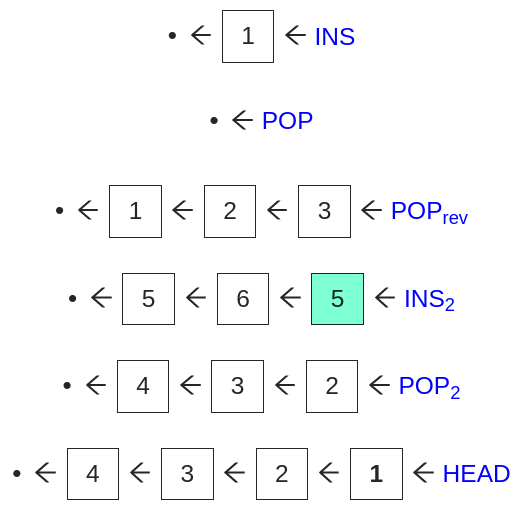
\includegraphics[width=0.8\textwidth]{stacks.png}
    \caption{The stacks view after performing some push operations on the queue.}
\end{figure}

\subsection{Individual Moves and Animations}

As discussed earlier, we would like to visualize each simple move in an operation. To do this, we needed our stacks view to process a \texttt{move} object and visualize it a nice way. First, we used the metadata in each move to provide an explanation of what the move does (i.e. what pointer operation or functional stack operation it does). For pushing, popping, and moving elements, we highlighted the appropriate elements in green/red and faded them in and out. 

For the moves for begin transfer and end transfer, the situation was slightly more complicated, since this consisted of assigning a pointer for a stack to another pointer. Originally, this resulted in a very abrupt visual change. We decided to split up end transfer into 3 moves, such that each move only made one stack assignment. We then highlighted all the elements that get ``added'' to the new stack in green, and highlighted the elements of the stack that get copied into the ``new stack'' in blue. After playing around with this effect, with the help of the explanatory text above it became quite clear that the operation was actually a single pointer assignment.

\begin{figure}[H]
    \centering
    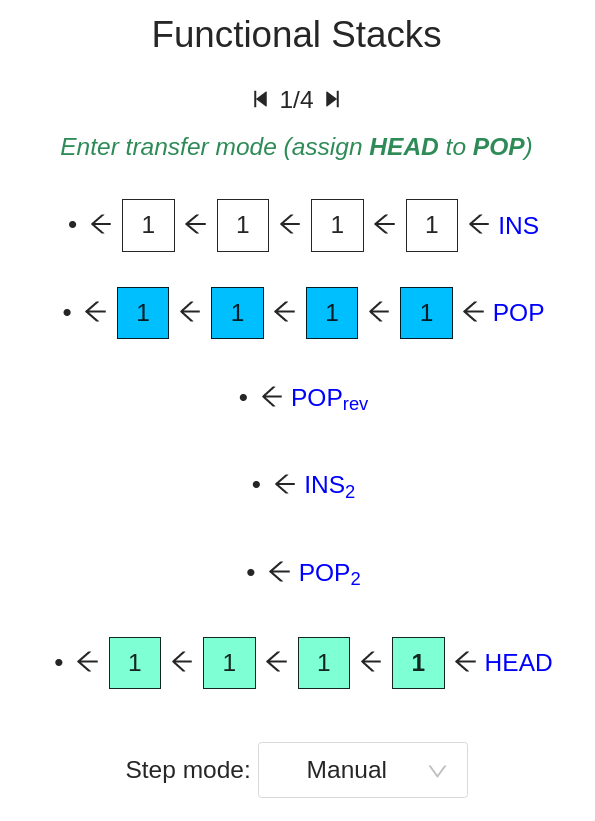
\includegraphics[width=0.6\textwidth]{highlight.png}
    \caption{The state of the stacks view when visualizing the move for begin transfer.}
\end{figure}


Finally, to navigate between the moves of each operation, we added three modes: manual, automatic, and skip to end. In manual mode, the user must use arrow buttons to go forwards/backwards between the moves. In automatic mode, we automatically step forward at regular intervals, and the pace is controlled by a speed slider. In skip to end mode, the queue immediately jumps to its final state after the operation.

\subsection{Version History}

The version history was more difficult than expected because of the large number of versions that are created. We eventually decided to implement both a linear version history and graph version history. Users can toggle a switch to choose which view they would like to see.

\subsubsection{Linear Version History}

In the linear version history, new versions are added to a bottom of a scrolling list of versions. When clicking on a version, all of its ancestors (the queues that were operated on to eventually create this version) are highlighted. The version history is written to mimic the style of pseudocode, and the user is able to see what operations created each queue and a list of elements for the current queue.

\begin{figure}[H]
    \centering
    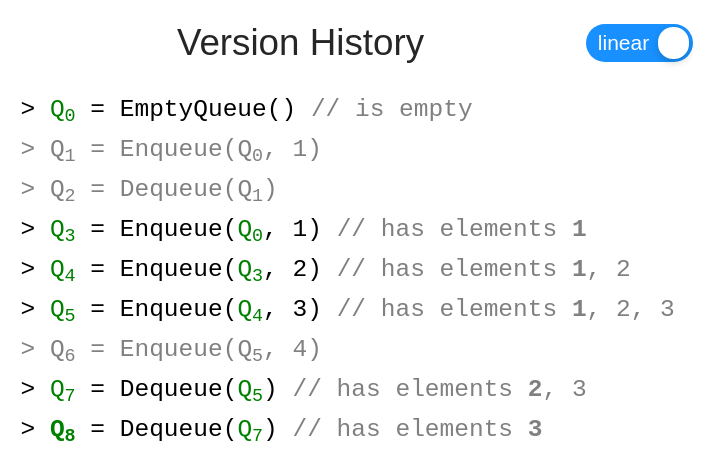
\includegraphics[width=0.6\textwidth]{linear.png}
    \caption{The linear version history view with version Q\textsubscript{8} selected.}
\end{figure}

\subsubsection{Graph Version History}

In the graph version history, each version is represented as a node. The versions are laid out vertically as a tree, where an edge connects a parent version to the child version that was created from the parent. Similar to the linear version history, the current version that is being displayed in the stack view is highlighted in green. Users can click on a different version to display a new version in the stack view and can perform enqueue/dequeue operations on the selected version. 

When the user hovers over a particular version with their mouse, a tooltip displaying the queue version number appears. This is particularly useful in identifying versions when there are so many nodes in the tree that they overlap. While we considered maintaining enough space between each node to prevent overlap, this came at the expense of the user having to scroll up and down the page to view different sections of the tree. We felt like the main benefit of the graph view was that a user can easily see the history of every version, and so seeing the entire graph at once without scrolling was important.

\begin{figure}[h!]
    \centering
    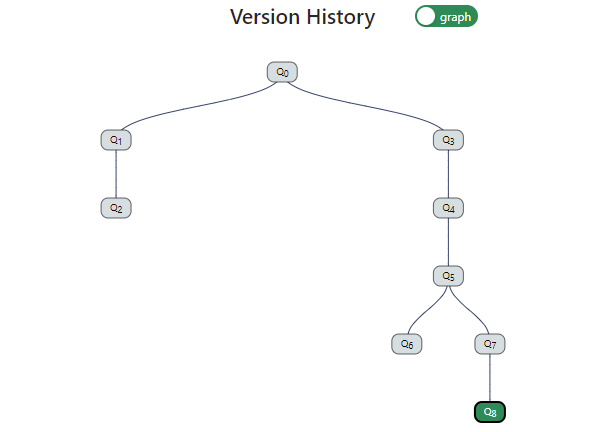
\includegraphics[width=.9\textwidth]{graph-version-history.PNG}
    \caption{The graph version history view with version Q\textsubscript{8} selected.}
\end{figure}

\subsection{Other Design Choices}

At the start of the project, as we were considering what language to base our code in, we decided between Python and JavaScript. While some of us had more experience with Python, we ultimately chose to code the project in JavaScript since it had better support with the framework and libraries we planned on using. In particular, we chose to use React since it allowed us to create an interactive UI with minimal setup time. Additionally, using React allowed us to take advantage of a UI library called Ant Design which is well-known its sleek, minimal icons and components. 

As we were developing the version history, we noticed that users would have to scroll back and forth from the version history at the bottom to the input \& stack view at the top. We ended up implementing a version where the stack view and version history were side-by-side so that users could see both at the same time, but in the end, decided to revert this change since we felt like the primary focus should be on the stack view. Having these two components next to each other minimized both of their horizontal real estate, and ended up causing users to have to scroll horizontally in order to get a sense of the stack structure.

%\todo{not necessary, but we could talk about the color scheme (seagreen chosen to not distract, etc) and/or why we chose react over other frameworks}

\section{Implementation details}
This interface is a React application with embedded Ant Design components and vanilla HTML/CSS/JavaScript. 

For the graph version of history, we used visx, a collection of low-level visualization primitives for React that build on top of D3.js. In particular, we used the visx tree example~\cite{vx-example} as a framework for our own code.

\subsection{Instructions for local setup}

This application requires that Node.js and npm be installed. Once npm is installed, the command \texttt{npm install yarn} can be run in order to install the package manager used to easily launch the code locally. The repository containing the code can be found at \href{https://github.com/6851-2021/functional-queue-visualization}{https://github.com/6851-2021/functional-queue-visualization}. Once it is cloned/downloaded, navigate to the \texttt{/app} directory, run \texttt{npm install} to install any package dependencies, and then run \texttt{yarn start} to launch the application. The app should open at \texttt{localhost:3000} in your browser. We recommend using Chrome as we primarily developed and tested using this browser. %\todo{were other browsers developed on?}

\section{Future Work}

As hinted at earlier, a really interesting additional feature would be to visualize the network of all pointers and nodes ever created, rather than just those relevant to the currently selected queue. This visualization could be done with an external library, similar to the graphical version history.

Internally, visualizing a queue takes $O(n)$ time, since we internally list all the elements of each stack and perform operations on them. The version history, as implemented, also takes $O(n)$. It would be interesting to try to update the visualizer's entire state in $O(1)$. However, since DOM operations will likely always be the bottleneck, it is unclear whether it would be possible to achieve significant performance improvements.

Overall, we are very happy with how this project has turned out and hope it can be published and put to good use in helping others understand how to implement functional queues in $O(1)$ per operation.

% visualization is not  O(1)
% showing hidden pointers 


% \section{Section Sample}
% \subsection{A Subsection Sample}
% Please note that the first paragraph of a section or subsection is
% not indented. The first paragraph that follows a table, figure,
% equation etc. does not need an indent, either.

% Subsequent paragraphs, however, are indented.

% \subsubsection{Sample Heading (Third Level)} Only two levels of
% headings should be numbered. Lower level headings remain unnumbered;
% they are formatted as run-in headings.

% \paragraph{Sample Heading (Fourth Level)}
% The contribution should contain no more than four levels of
% headings. Table~\ref{tab1} gives a summary of all heading levels.

% \begin{table}
% \caption{Table captions should be placed above the
% tables.}\label{tab1}
% \begin{tabular}{|l|l|l|}
% \hline
% Heading level &  Example & Font size and style\\
% \hline
% Title (centered) &  {\Large\bfseries Lecture Notes} & 14 point, bold\\
% 1st-level heading &  {\large\bfseries 1 Introduction} & 12 point, bold\\
% 2nd-level heading & {\bfseries 2.1 Printing Area} & 10 point, bold\\
% 3rd-level heading & {\bfseries Run-in Heading in Bold.} Text follows & 10 point, bold\\
% 4th-level heading & {\itshape Lowest Level Heading.} Text follows & 10 point, italic\\
% \hline
% \end{tabular}
% \end{table}


% \noindent Displayed equations are centered and set on a separate
% line.
% \begin{equation}
% x + y = z
% \end{equation}
% Please try to avoid rasterized images for line-art diagrams and
% schemas. Whenever possible, use vector graphics instead (see
% Fig.~\ref{fig1}).

% \lipsum[44]

% \begin{figure}
% \includegraphics[width=\textwidth]{fig1.eps}
% \caption{A figure caption is always placed below the illustration.
% Please note that short captions are centered, while long ones are
% justified by the macro package automatically.} \label{fig1}
% \end{figure}

%
% ---- Bibliography ----
%
% BibTeX users should specify bibliography style 'splncs04'.
% References will then be sorted and formatted in the correct style.
%
\bibliographystyle{refs-style}
\bibliography{refs}
%
\end{document}
